\documentclass[11pt,]{article}
\usepackage{lmodern}
\usepackage{amssymb,amsmath}
\usepackage{ifxetex,ifluatex}
\usepackage{fixltx2e} % provides \textsubscript
\ifnum 0\ifxetex 1\fi\ifluatex 1\fi=0 % if pdftex
  \usepackage[T1]{fontenc}
  \usepackage[utf8]{inputenc}
\else % if luatex or xelatex
  \ifxetex
    \usepackage{mathspec}
  \else
    \usepackage{fontspec}
  \fi
  \defaultfontfeatures{Ligatures=TeX,Scale=MatchLowercase}
\fi
% use upquote if available, for straight quotes in verbatim environments
\IfFileExists{upquote.sty}{\usepackage{upquote}}{}
% use microtype if available
\IfFileExists{microtype.sty}{%
\usepackage{microtype}
\UseMicrotypeSet[protrusion]{basicmath} % disable protrusion for tt fonts
}{}
\usepackage[margin=1in]{geometry}
\usepackage{hyperref}
\hypersetup{unicode=true,
            pdftitle={Package vars},
            pdfauthor={Paul GUILLOTTE \& Jules CORBEL},
            pdfborder={0 0 0},
            breaklinks=true}
\urlstyle{same}  % don't use monospace font for urls
\usepackage{color}
\usepackage{fancyvrb}
\newcommand{\VerbBar}{|}
\newcommand{\VERB}{\Verb[commandchars=\\\{\}]}
\DefineVerbatimEnvironment{Highlighting}{Verbatim}{commandchars=\\\{\}}
% Add ',fontsize=\small' for more characters per line
\usepackage{framed}
\definecolor{shadecolor}{RGB}{248,248,248}
\newenvironment{Shaded}{\begin{snugshade}}{\end{snugshade}}
\newcommand{\KeywordTok}[1]{\textcolor[rgb]{0.13,0.29,0.53}{\textbf{#1}}}
\newcommand{\DataTypeTok}[1]{\textcolor[rgb]{0.13,0.29,0.53}{#1}}
\newcommand{\DecValTok}[1]{\textcolor[rgb]{0.00,0.00,0.81}{#1}}
\newcommand{\BaseNTok}[1]{\textcolor[rgb]{0.00,0.00,0.81}{#1}}
\newcommand{\FloatTok}[1]{\textcolor[rgb]{0.00,0.00,0.81}{#1}}
\newcommand{\ConstantTok}[1]{\textcolor[rgb]{0.00,0.00,0.00}{#1}}
\newcommand{\CharTok}[1]{\textcolor[rgb]{0.31,0.60,0.02}{#1}}
\newcommand{\SpecialCharTok}[1]{\textcolor[rgb]{0.00,0.00,0.00}{#1}}
\newcommand{\StringTok}[1]{\textcolor[rgb]{0.31,0.60,0.02}{#1}}
\newcommand{\VerbatimStringTok}[1]{\textcolor[rgb]{0.31,0.60,0.02}{#1}}
\newcommand{\SpecialStringTok}[1]{\textcolor[rgb]{0.31,0.60,0.02}{#1}}
\newcommand{\ImportTok}[1]{#1}
\newcommand{\CommentTok}[1]{\textcolor[rgb]{0.56,0.35,0.01}{\textit{#1}}}
\newcommand{\DocumentationTok}[1]{\textcolor[rgb]{0.56,0.35,0.01}{\textbf{\textit{#1}}}}
\newcommand{\AnnotationTok}[1]{\textcolor[rgb]{0.56,0.35,0.01}{\textbf{\textit{#1}}}}
\newcommand{\CommentVarTok}[1]{\textcolor[rgb]{0.56,0.35,0.01}{\textbf{\textit{#1}}}}
\newcommand{\OtherTok}[1]{\textcolor[rgb]{0.56,0.35,0.01}{#1}}
\newcommand{\FunctionTok}[1]{\textcolor[rgb]{0.00,0.00,0.00}{#1}}
\newcommand{\VariableTok}[1]{\textcolor[rgb]{0.00,0.00,0.00}{#1}}
\newcommand{\ControlFlowTok}[1]{\textcolor[rgb]{0.13,0.29,0.53}{\textbf{#1}}}
\newcommand{\OperatorTok}[1]{\textcolor[rgb]{0.81,0.36,0.00}{\textbf{#1}}}
\newcommand{\BuiltInTok}[1]{#1}
\newcommand{\ExtensionTok}[1]{#1}
\newcommand{\PreprocessorTok}[1]{\textcolor[rgb]{0.56,0.35,0.01}{\textit{#1}}}
\newcommand{\AttributeTok}[1]{\textcolor[rgb]{0.77,0.63,0.00}{#1}}
\newcommand{\RegionMarkerTok}[1]{#1}
\newcommand{\InformationTok}[1]{\textcolor[rgb]{0.56,0.35,0.01}{\textbf{\textit{#1}}}}
\newcommand{\WarningTok}[1]{\textcolor[rgb]{0.56,0.35,0.01}{\textbf{\textit{#1}}}}
\newcommand{\AlertTok}[1]{\textcolor[rgb]{0.94,0.16,0.16}{#1}}
\newcommand{\ErrorTok}[1]{\textcolor[rgb]{0.64,0.00,0.00}{\textbf{#1}}}
\newcommand{\NormalTok}[1]{#1}
\usepackage{longtable,booktabs}
\usepackage{graphicx,grffile}
\makeatletter
\def\maxwidth{\ifdim\Gin@nat@width>\linewidth\linewidth\else\Gin@nat@width\fi}
\def\maxheight{\ifdim\Gin@nat@height>\textheight\textheight\else\Gin@nat@height\fi}
\makeatother
% Scale images if necessary, so that they will not overflow the page
% margins by default, and it is still possible to overwrite the defaults
% using explicit options in \includegraphics[width, height, ...]{}
\setkeys{Gin}{width=\maxwidth,height=\maxheight,keepaspectratio}
\IfFileExists{parskip.sty}{%
\usepackage{parskip}
}{% else
\setlength{\parindent}{0pt}
\setlength{\parskip}{6pt plus 2pt minus 1pt}
}
\setlength{\emergencystretch}{3em}  % prevent overfull lines
\providecommand{\tightlist}{%
  \setlength{\itemsep}{0pt}\setlength{\parskip}{0pt}}
\setcounter{secnumdepth}{5}
% Redefines (sub)paragraphs to behave more like sections
\ifx\paragraph\undefined\else
\let\oldparagraph\paragraph
\renewcommand{\paragraph}[1]{\oldparagraph{#1}\mbox{}}
\fi
\ifx\subparagraph\undefined\else
\let\oldsubparagraph\subparagraph
\renewcommand{\subparagraph}[1]{\oldsubparagraph{#1}\mbox{}}
\fi

%%% Use protect on footnotes to avoid problems with footnotes in titles
\let\rmarkdownfootnote\footnote%
\def\footnote{\protect\rmarkdownfootnote}

%%% Change title format to be more compact
\usepackage{titling}

% Create subtitle command for use in maketitle
\newcommand{\subtitle}[1]{
  \posttitle{
    \begin{center}\large#1\end{center}
    }
}

\setlength{\droptitle}{-2em}

  \title{Package vars}
    \pretitle{\vspace{\droptitle}\centering\huge}
  \posttitle{\par}
    \author{Paul GUILLOTTE \& Jules CORBEL}
    \preauthor{\centering\large\emph}
  \postauthor{\par}
      \predate{\centering\large\emph}
  \postdate{\par}
    \date{01/02/2019}


\begin{document}
\maketitle
\begin{abstract}
bbbbb
\end{abstract}

{
\setcounter{tocdepth}{2}
\tableofcontents
}
\section*{Introduction}\label{introduction}
\addcontentsline{toc}{section}{Introduction}

\section{Analyse descriptive des
séries}\label{analyse-descriptive-des-series}

\subsection{Rappel sur la stationnarité du second
ordre}\label{rappel-sur-la-stationnarite-du-second-ordre}

Avant de commencer à analyser les séries, nous rappelons des bases sur
des notions dont nous aurons besoin par la suite.

Dans de nombreux modèles de séries temporelles, la série en entrée doit
satisfaire une hypothèse de stationnarité. Les conditions de la
stationnarité du second ordre.

\(E[y_{t}]=\mu \forall t=1...T\)

\(Var[y_{t}]=\sigma ^{2}\neq \infty \forall t=1...t Var[y_{t}]=\sigma ^{2}\neq \infty \forall i=1...T\)

\(Cov[y_{i},Z_{i-k}]=f(k) \forall i=1...t, \forall k=1...t\)

Nous nous intéressons dans cette partie aux différentes séries
trimestrielles à notre disposition. Dans un premier temps, nous nous
intéressons aux corrélations entre les variables deux à deux afin de
nous faire une première idée du lien qu'il existe entre les variables.

\subsection{\texorpdfstring{Masse salariale
\label{MSE}}{Masse salariale }}\label{masse-salariale}

\begin{Shaded}
\begin{Highlighting}[]
\NormalTok{  MSE <-}\StringTok{ }\KeywordTok{ts}\NormalTok{(trim}\OperatorTok{$}\NormalTok{MSE, }\DataTypeTok{start =} \DecValTok{1990}\NormalTok{, }\DataTypeTok{end =} \KeywordTok{c}\NormalTok{(}\DecValTok{2017}\NormalTok{, }\DecValTok{2}\NormalTok{), }\DataTypeTok{frequency=}\DecValTok{4}\NormalTok{)}
  \KeywordTok{plot}\NormalTok{(MSE, }\DataTypeTok{main=}\StringTok{"Evolution trimestrielle de la masse salariale"}\NormalTok{, }\DataTypeTok{xaxt=}\StringTok{"n"}\NormalTok{, }\DataTypeTok{cex.main=}\FloatTok{0.9}\NormalTok{)}
  \KeywordTok{axis}\NormalTok{(}\DataTypeTok{side=}\DecValTok{1}\NormalTok{, }\DataTypeTok{at=}\KeywordTok{seq}\NormalTok{(}\DecValTok{1990}\NormalTok{,}\DecValTok{2015}\NormalTok{,}\DecValTok{5}\NormalTok{), }\DataTypeTok{labels=}\KeywordTok{c}\NormalTok{(}\StringTok{"1990Q1"}\NormalTok{, }\StringTok{"1995Q1"}\NormalTok{, }\StringTok{"2000Q1"}\NormalTok{, }\StringTok{"2005Q1"}\NormalTok{, }
                                             \StringTok{"2010Q1"}\NormalTok{, }\StringTok{"2015Q1"}\NormalTok{))}
\end{Highlighting}
\end{Shaded}

\begin{figure}

{\centering 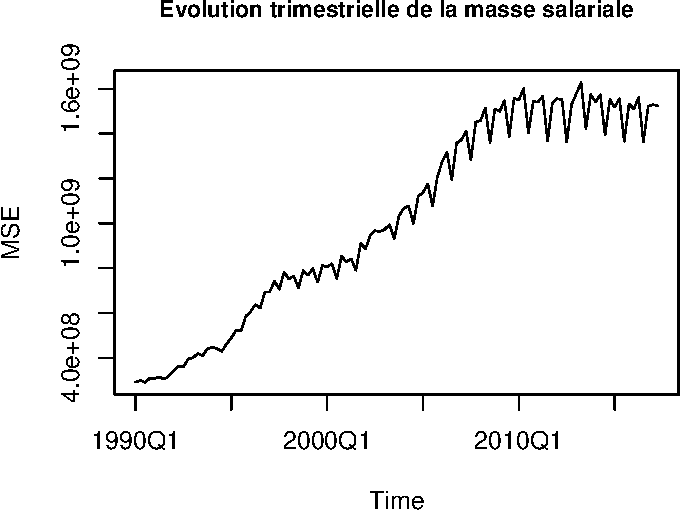
\includegraphics{doc_files/figure-latex/unnamed-chunk-1-1} 

}

\caption{\label{fig1}}\label{fig:unnamed-chunk-1}
\end{figure}

\begin{Shaded}
\begin{Highlighting}[]
  \KeywordTok{par}\NormalTok{(}\DataTypeTok{mfrow=}\KeywordTok{c}\NormalTok{(}\DecValTok{1}\NormalTok{,}\DecValTok{2}\NormalTok{), }\DataTypeTok{cex.main=}\FloatTok{0.8}\NormalTok{)}
  \KeywordTok{acf}\NormalTok{(MSE, }\DataTypeTok{main=}\StringTok{"Auto-corrélation de la}
\StringTok{      masse salariale trimestrielle"}\NormalTok{, }\DataTypeTok{lag.max=}\DecValTok{20}\NormalTok{)}
  \KeywordTok{pacf}\NormalTok{(MSE, }\DataTypeTok{main=}\StringTok{"Autocorrélation partielle}
\StringTok{       de la masse salariale trimestrielle"}\NormalTok{, }\DataTypeTok{lag.max=}\DecValTok{20}\NormalTok{)}
\end{Highlighting}
\end{Shaded}

\begin{figure}
\centering
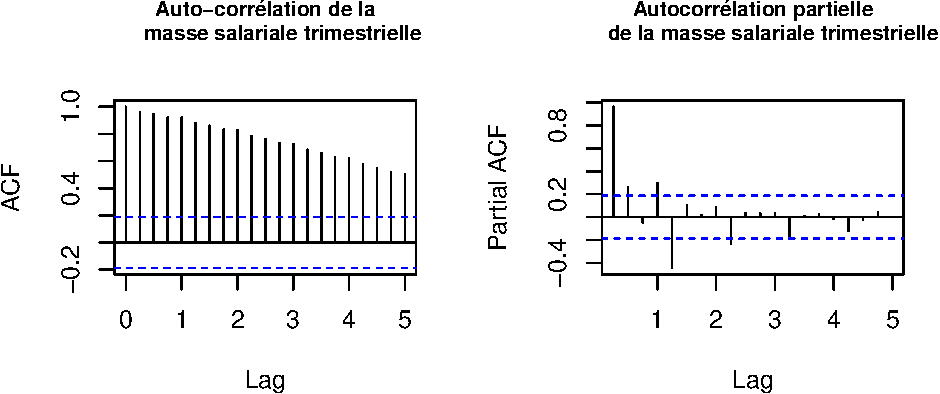
\includegraphics{doc_files/figure-latex/unnamed-chunk-2-1.pdf}
\caption{\label{fig2}}
\end{figure}

\begin{Shaded}
\begin{Highlighting}[]
  \KeywordTok{kpss.test}\NormalTok{(MSE)}
\end{Highlighting}
\end{Shaded}

\begin{verbatim}
## Warning in kpss.test(MSE): p-value smaller than printed p-value
\end{verbatim}

\begin{verbatim}
## 
##  KPSS Test for Level Stationarity
## 
## data:  MSE
## KPSS Level = 3.6772, Truncation lag parameter = 2, p-value = 0.01
\end{verbatim}

\begin{Shaded}
\begin{Highlighting}[]
  \KeywordTok{adf.test}\NormalTok{(MSE)}
\end{Highlighting}
\end{Shaded}

\begin{verbatim}
## Warning in adf.test(MSE): p-value greater than printed p-value
\end{verbatim}

\begin{verbatim}
## 
##  Augmented Dickey-Fuller Test
## 
## data:  MSE
## Dickey-Fuller = -0.20821, Lag order = 4, p-value = 0.99
## alternative hypothesis: stationary
\end{verbatim}

La masse salariale trimestrielle, représentée en Figure \ref{fig1}
possède une composante de tendance de 1990 à 2010. La série tend par la
suite à stagner. Nous remarquons également une saisonnalité sur cette
série, qui est de plus en plus marquée à mesure que le temps passe.

Comme la série comporte une tendance et une saisonnalité, elle ne
correspond pas aux deux premières conditions de la stationnarité du
second ordre, soit que la série possède une moyenne et un écart-type
constants. Cela est confirmé par la Figure \ref{fig2}, qui nous montre
fonction ACF qui décroît régulièrement. Nous effectuons également un
test de KPSS (test de stationnarité) servant à vérifier si la série est
stationnaire ou non (sous l'hypothèse \(H_{0}\) la série est
stationnaire, et sous l'hypothèse \(H_{1}\) elle ne l'est pas). La série
est dite stationnaire si ses propriétés statistiques (espérance,
variance et auto-corrélation) sont fixes au cours du temps. La p-value
est de 0.01 ce qui nous confirme que la série n'est pas stationnaire
avec un risque de première espèce de 5\%. Nous mettons également en
place un test de racines unitaires, le test de Dickey Fuller augmenté.
Son hypothèse nulle est que la série a été générée par un processus
présentant une racine unitaire, et donc que la série n'est pas
stationnaire. Ici, avec un risque de premier espèce à 5\%, on conserve
l'hypothèse nulle est on conclut, à l'aide des deux tests effectués, que
la série n'est pas stationnaire.

\subsection{\texorpdfstring{PIB \label{PIB}}{PIB }}\label{pib}

\begin{Shaded}
\begin{Highlighting}[]
\NormalTok{  PIB <-}\StringTok{ }\KeywordTok{ts}\NormalTok{(trim}\OperatorTok{$}\NormalTok{PIB, }\DataTypeTok{start =} \DecValTok{1990}\NormalTok{, }\DataTypeTok{end =} \KeywordTok{c}\NormalTok{(}\DecValTok{2017}\NormalTok{, }\DecValTok{1}\NormalTok{), }\DataTypeTok{frequency=}\DecValTok{4}\NormalTok{)}
  \KeywordTok{plot}\NormalTok{(PIB, }\DataTypeTok{main=}\StringTok{"Evolution trimestrielle du PIB"}\NormalTok{,}\DataTypeTok{xaxt=}\StringTok{"n"}\NormalTok{, }\DataTypeTok{cex.main=}\FloatTok{0.9}\NormalTok{)}
  \KeywordTok{axis}\NormalTok{(}\DataTypeTok{side=}\DecValTok{1}\NormalTok{, }\DataTypeTok{at=}\KeywordTok{seq}\NormalTok{(}\DecValTok{1990}\NormalTok{,}\DecValTok{2015}\NormalTok{,}\DecValTok{5}\NormalTok{), }\DataTypeTok{labels=}\KeywordTok{c}\NormalTok{(}\StringTok{"1990Q1"}\NormalTok{, }\StringTok{"1995Q1"}\NormalTok{, }\StringTok{"2000Q1"}\NormalTok{, }\StringTok{"2005Q1"}\NormalTok{, }\StringTok{"2010Q1"}\NormalTok{, }\StringTok{"2015Q1"}\NormalTok{))}
\end{Highlighting}
\end{Shaded}

\begin{figure}

{\centering 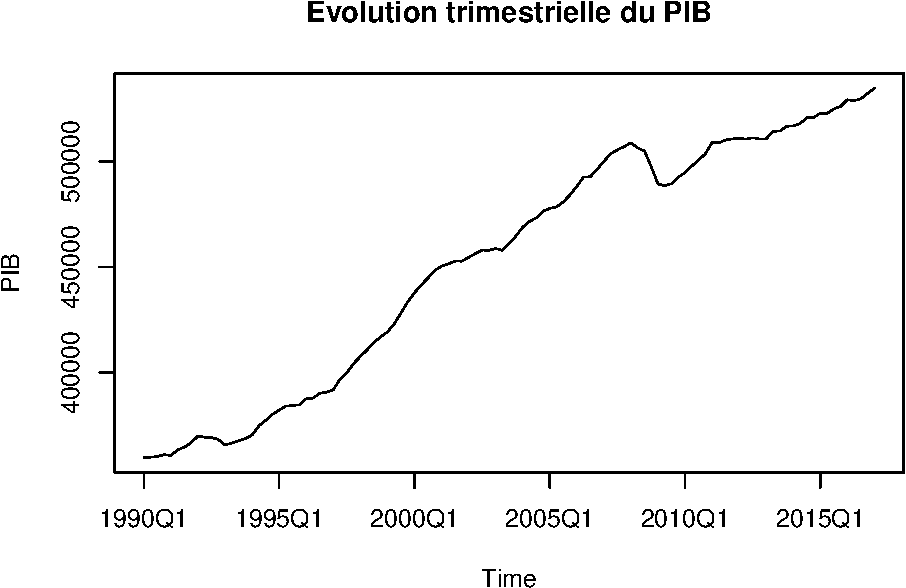
\includegraphics{doc_files/figure-latex/unnamed-chunk-3-1} 

}

\caption{\label{fig3}}\label{fig:unnamed-chunk-3}
\end{figure}

\begin{Shaded}
\begin{Highlighting}[]
  \KeywordTok{par}\NormalTok{(}\DataTypeTok{mfrow=}\KeywordTok{c}\NormalTok{(}\DecValTok{1}\NormalTok{,}\DecValTok{2}\NormalTok{), }\DataTypeTok{cex.main=}\FloatTok{0.8}\NormalTok{)}
  \KeywordTok{acf}\NormalTok{(PIB, }\DataTypeTok{main=}\StringTok{"Auto-corrélation }
\StringTok{      du PIB trimestriel"}\NormalTok{, }\DataTypeTok{lag.max=}\DecValTok{40}\NormalTok{)}
  \KeywordTok{pacf}\NormalTok{(PIB, }\DataTypeTok{main=}\StringTok{"Autocorrélation partielle}
\StringTok{       du PIB trimestriel"}\NormalTok{, }\DataTypeTok{lag.max=}\DecValTok{40}\NormalTok{)}
\end{Highlighting}
\end{Shaded}

\begin{figure}
\centering
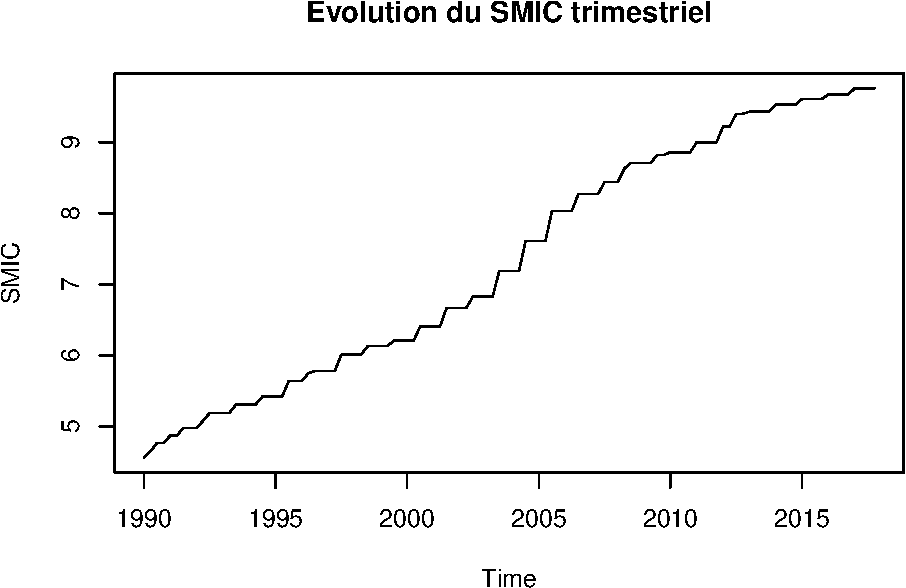
\includegraphics{doc_files/figure-latex/unnamed-chunk-4-1.pdf}
\caption{\label{fig4}}
\end{figure}

\begin{Shaded}
\begin{Highlighting}[]
  \KeywordTok{par}\NormalTok{(}\DataTypeTok{mfrow=}\KeywordTok{c}\NormalTok{(}\DecValTok{1}\NormalTok{,}\DecValTok{1}\NormalTok{))}
  \KeywordTok{kpss.test}\NormalTok{(PIB)}
\end{Highlighting}
\end{Shaded}

\begin{verbatim}
## Warning in kpss.test(PIB): p-value smaller than printed p-value
\end{verbatim}

\begin{verbatim}
## 
##  KPSS Test for Level Stationarity
## 
## data:  PIB
## KPSS Level = 3.6473, Truncation lag parameter = 2, p-value = 0.01
\end{verbatim}

\begin{Shaded}
\begin{Highlighting}[]
  \KeywordTok{adf.test}\NormalTok{(PIB)}
\end{Highlighting}
\end{Shaded}

\begin{verbatim}
## 
##  Augmented Dickey-Fuller Test
## 
## data:  PIB
## Dickey-Fuller = -1.3274, Lag order = 4, p-value = 0.8557
## alternative hypothesis: stationary
\end{verbatim}

La Figure \ref{fig3} nous montre le PIB trimestriel qui, comme pour la
masse salarialepossède une tendance. Cependant, il ne semble pas
posséder de saisonnalité. Cette série ne semble donc pas non plus
stationnaire. Nous effectuons à nouveau un test de KPSS. La p-value est
de 0.01 ce qui nous confirme que la série n'est pas stationnaire avec un
risque de première espèce de 5\%. Même conclusion au regard du test
augmenté de Dickey Fuller.

\subsection{SMIC}\label{smic}

\begin{Shaded}
\begin{Highlighting}[]
\NormalTok{  SMIC <-}\StringTok{ }\KeywordTok{ts}\NormalTok{(trim}\OperatorTok{$}\NormalTok{SMIC, }\DataTypeTok{start =} \KeywordTok{c}\NormalTok{(}\DecValTok{1990}\NormalTok{,}\DecValTok{1}\NormalTok{), }\DataTypeTok{end =} \KeywordTok{c}\NormalTok{(}\DecValTok{2017}\NormalTok{, }\DecValTok{4}\NormalTok{), }\DataTypeTok{frequency =} \DecValTok{4}\NormalTok{)}
  \KeywordTok{plot}\NormalTok{(SMIC, }\DataTypeTok{main=}\StringTok{"Evolution trimestrielle du SMIC"}\NormalTok{, }\DataTypeTok{xaxt=}\StringTok{"n"}\NormalTok{, }\DataTypeTok{cex.main=}\FloatTok{0.9}\NormalTok{)}
  \KeywordTok{axis}\NormalTok{(}\DataTypeTok{side=}\DecValTok{1}\NormalTok{, }\DataTypeTok{at=}\KeywordTok{seq}\NormalTok{(}\DecValTok{1990}\NormalTok{,}\DecValTok{2015}\NormalTok{,}\DecValTok{5}\NormalTok{), }\DataTypeTok{labels=}\KeywordTok{c}\NormalTok{(}\StringTok{"1990Q1"}\NormalTok{, }\StringTok{"1995Q1"}\NormalTok{, }\StringTok{"2000Q1"}\NormalTok{, }\StringTok{"2005Q1"}\NormalTok{, }\StringTok{"2010Q1"}\NormalTok{, }\StringTok{"2015Q1"}\NormalTok{))}
\end{Highlighting}
\end{Shaded}

\begin{figure}

{\centering 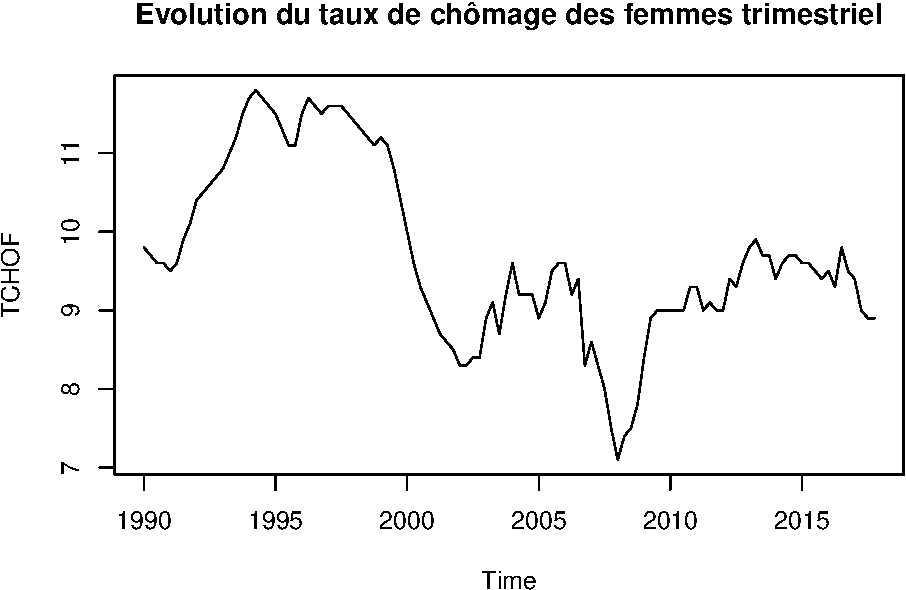
\includegraphics{doc_files/figure-latex/unnamed-chunk-5-1} 

}

\caption{\label{fig5}}\label{fig:unnamed-chunk-5}
\end{figure}

\begin{Shaded}
\begin{Highlighting}[]
  \KeywordTok{par}\NormalTok{(}\DataTypeTok{mfrow=}\KeywordTok{c}\NormalTok{(}\DecValTok{1}\NormalTok{,}\DecValTok{2}\NormalTok{), }\DataTypeTok{cex.main=}\FloatTok{0.8}\NormalTok{)}
  \KeywordTok{acf}\NormalTok{(SMIC, }\DataTypeTok{main=}\StringTok{"Auto-corrélation du}
\StringTok{      SMIC trimestriel"}\NormalTok{, }\DataTypeTok{lag.max=}\DecValTok{20}\NormalTok{)}
  \KeywordTok{pacf}\NormalTok{(SMIC, }\DataTypeTok{main=}\StringTok{"Autocorrélation partielle}
\StringTok{       du SMIC trimestriel"}\NormalTok{, }\DataTypeTok{lag.max=}\DecValTok{20}\NormalTok{)}
\end{Highlighting}
\end{Shaded}

\begin{figure}
\centering
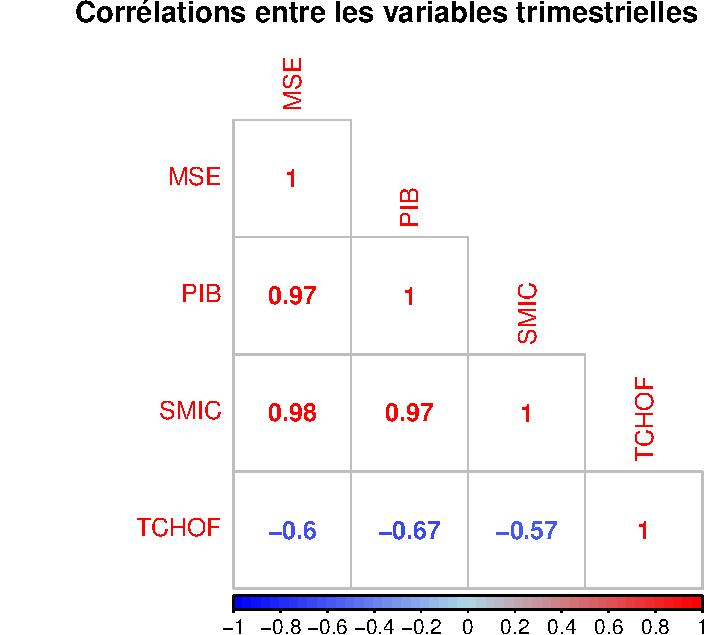
\includegraphics{doc_files/figure-latex/unnamed-chunk-6-1.pdf}
\caption{\label{fig6}}
\end{figure}

\begin{Shaded}
\begin{Highlighting}[]
  \KeywordTok{par}\NormalTok{(}\DataTypeTok{mfrow=}\KeywordTok{c}\NormalTok{(}\DecValTok{1}\NormalTok{,}\DecValTok{1}\NormalTok{))}
  \KeywordTok{kpss.test}\NormalTok{(SMIC)}
\end{Highlighting}
\end{Shaded}

\begin{verbatim}
## Warning in kpss.test(SMIC): p-value smaller than printed p-value
\end{verbatim}

\begin{verbatim}
## 
##  KPSS Test for Level Stationarity
## 
## data:  SMIC
## KPSS Level = 3.8382, Truncation lag parameter = 2, p-value = 0.01
\end{verbatim}

\begin{Shaded}
\begin{Highlighting}[]
  \KeywordTok{adf.test}\NormalTok{(SMIC)}
\end{Highlighting}
\end{Shaded}

\begin{verbatim}
## 
##  Augmented Dickey-Fuller Test
## 
## data:  SMIC
## Dickey-Fuller = -1.4174, Lag order = 4, p-value = 0.8184
## alternative hypothesis: stationary
\end{verbatim}

Au regard de la Figure \ref{fig5}, on s'aperçoit qu'il y a bien une
tendance. Pour la saisonnalité, il est plus difficile de savoir s'il en
existe une ou pas, puisque la série semble augmenter seulement à
certains temps. Les tests de KPSS et de Dickey Fuller augmenté nous
confirment que la série n'est pas stationnaire.

\subsection{\texorpdfstring{Taux de chômage des femmes
\label{TCHOF}}{Taux de chômage des femmes }}\label{taux-de-chomage-des-femmes}

\begin{Shaded}
\begin{Highlighting}[]
\NormalTok{  TCHOF <-}\StringTok{ }\KeywordTok{ts}\NormalTok{(trim}\OperatorTok{$}\NormalTok{TCHOF, }\DataTypeTok{start =} \KeywordTok{c}\NormalTok{(}\DecValTok{1990}\NormalTok{,}\DecValTok{1}\NormalTok{), }\DataTypeTok{end =} \KeywordTok{c}\NormalTok{(}\DecValTok{2017}\NormalTok{, }\DecValTok{4}\NormalTok{), }\DataTypeTok{frequency =} \DecValTok{4}\NormalTok{)}
  \KeywordTok{plot}\NormalTok{(TCHOF, }\DataTypeTok{main=}\StringTok{"Evolution trimestrielle du taux de chômage des femmes"}\NormalTok{, }\DataTypeTok{xaxt=}\StringTok{"n"}\NormalTok{, }\DataTypeTok{cex.main=}\FloatTok{0.9}\NormalTok{)}
  \KeywordTok{axis}\NormalTok{(}\DataTypeTok{side=}\DecValTok{1}\NormalTok{, }\DataTypeTok{at=}\KeywordTok{seq}\NormalTok{(}\DecValTok{1990}\NormalTok{,}\DecValTok{2015}\NormalTok{,}\DecValTok{5}\NormalTok{), }\DataTypeTok{labels=}\KeywordTok{c}\NormalTok{(}\StringTok{"1990Q1"}\NormalTok{, }\StringTok{"1995Q1"}\NormalTok{, }\StringTok{"2000Q1"}\NormalTok{, }\StringTok{"2005Q1"}\NormalTok{, }\StringTok{"2010Q1"}\NormalTok{, }\StringTok{"2015Q1"}\NormalTok{))}
\end{Highlighting}
\end{Shaded}

\begin{figure}

{\centering 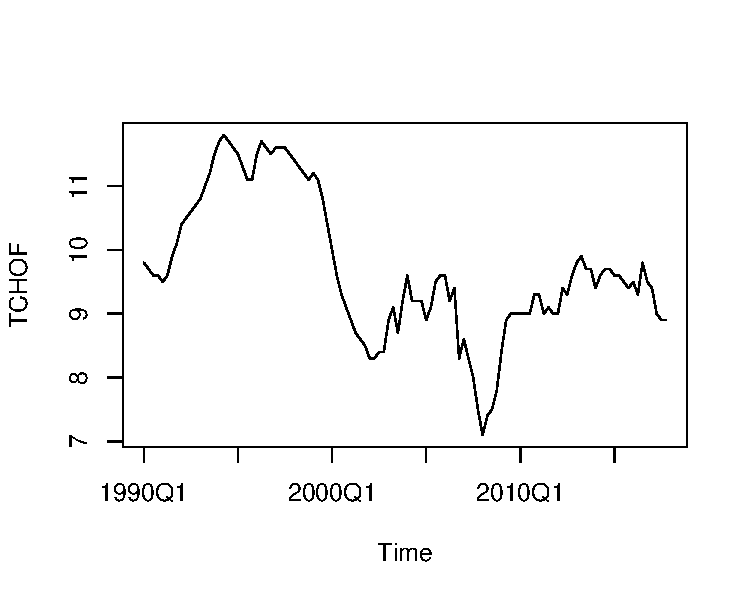
\includegraphics{doc_files/figure-latex/unnamed-chunk-7-1} 

}

\caption{\label{fig7}}\label{fig:unnamed-chunk-7}
\end{figure}

\begin{Shaded}
\begin{Highlighting}[]
  \KeywordTok{par}\NormalTok{(}\DataTypeTok{mfrow=}\KeywordTok{c}\NormalTok{(}\DecValTok{1}\NormalTok{,}\DecValTok{2}\NormalTok{), }\DataTypeTok{cex.main=}\FloatTok{0.8}\NormalTok{)}
  \KeywordTok{acf}\NormalTok{(TCHOF, }\DataTypeTok{main=}\StringTok{"Auto-corrélation du taux de}
\StringTok{      chômage des femmes trimestriel"}\NormalTok{, }\DataTypeTok{lag.max=}\DecValTok{20}\NormalTok{)}
  \KeywordTok{pacf}\NormalTok{(TCHOF, }\DataTypeTok{main=}\StringTok{"Autocorrélation partielle du}
\StringTok{       taux de chômage des femmes trimestriel"}\NormalTok{, }\DataTypeTok{lag.max=}\DecValTok{20}\NormalTok{)}
\end{Highlighting}
\end{Shaded}

\begin{figure}
\centering
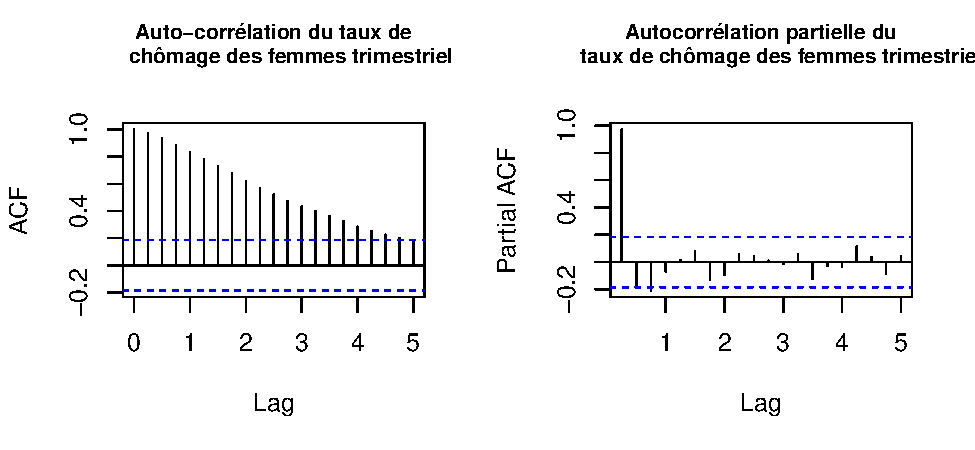
\includegraphics{doc_files/figure-latex/unnamed-chunk-8-1.pdf}
\caption{\label{fig8}}
\end{figure}

\begin{Shaded}
\begin{Highlighting}[]
  \KeywordTok{par}\NormalTok{(}\DataTypeTok{mfrow=}\KeywordTok{c}\NormalTok{(}\DecValTok{1}\NormalTok{,}\DecValTok{1}\NormalTok{))}
  \KeywordTok{kpss.test}\NormalTok{(TCHOF)}
\end{Highlighting}
\end{Shaded}

\begin{verbatim}
## Warning in kpss.test(TCHOF): p-value smaller than printed p-value
\end{verbatim}

\begin{verbatim}
## 
##  KPSS Test for Level Stationarity
## 
## data:  TCHOF
## KPSS Level = 1.6407, Truncation lag parameter = 2, p-value = 0.01
\end{verbatim}

\begin{Shaded}
\begin{Highlighting}[]
  \KeywordTok{adf.test}\NormalTok{(TCHOF)}
\end{Highlighting}
\end{Shaded}

\begin{verbatim}
## 
##  Augmented Dickey-Fuller Test
## 
## data:  TCHOF
## Dickey-Fuller = -2.5838, Lag order = 4, p-value = 0.3344
## alternative hypothesis: stationary
\end{verbatim}

Pour cette dernière série (Figure \ref{fig7}) qui représente le taux de
chômage trimestriel des femmes, il ne semble pas y avoir de
saisonnalité. On remarque cependant qu'il y a bien une tendance, au
regard de la Figure \ref{fig8}. En regardant la série de plus près, on
s'aperçoit que la tendance semble être ``par morceaux'' : d'abord une
hausse de 1990 à 1996, puis elle décroît jusqu'en 2002, avant
d'augmenter à nouveau jusqu'en 2007, de chuter jusqu'en 2010. Si la
série ne possède pas une tendance uniforme sur toute la durée étudiée,
elle semble donc bien posséder une tendance par morceaux. Les tests KPSS
et de Dickey Fuller augmenté nous confirment que la série n'est pas
stationnaire, avec un risque de première espèce de 5\%.

\subsection{Calcul des corrélations}\label{calcul-des-correlations}

\begin{Shaded}
\begin{Highlighting}[]
\KeywordTok{corrplot}\NormalTok{(}\KeywordTok{cor}\NormalTok{(trim[}\DecValTok{1}\OperatorTok{:}\DecValTok{109}\NormalTok{,}\OperatorTok{-}\DecValTok{1}\NormalTok{]), }\DataTypeTok{method =} \StringTok{"number"}\NormalTok{, }\DataTypeTok{type=}\StringTok{"lower"}\NormalTok{,}
         \DataTypeTok{p.mat=}\KeywordTok{cor.mtest}\NormalTok{(trim[}\DecValTok{1}\OperatorTok{:}\DecValTok{109}\NormalTok{,}\OperatorTok{-}\DecValTok{1}\NormalTok{], }\FloatTok{0.95}\NormalTok{)[[}\DecValTok{1}\NormalTok{]], }\DataTypeTok{insig=}\StringTok{"pch"}\NormalTok{,}
         \DataTypeTok{col=}\KeywordTok{colorRampPalette}\NormalTok{(}\KeywordTok{c}\NormalTok{(}\StringTok{"blue"}\NormalTok{, }\StringTok{"light blue"}\NormalTok{, }\StringTok{"red"}\NormalTok{))(}\DecValTok{50}\NormalTok{), }\DataTypeTok{title =} \StringTok{"}
\StringTok{         Corrélations entre les variables trimestrielles"}\NormalTok{)}
\end{Highlighting}
\end{Shaded}

\begin{figure}
\centering
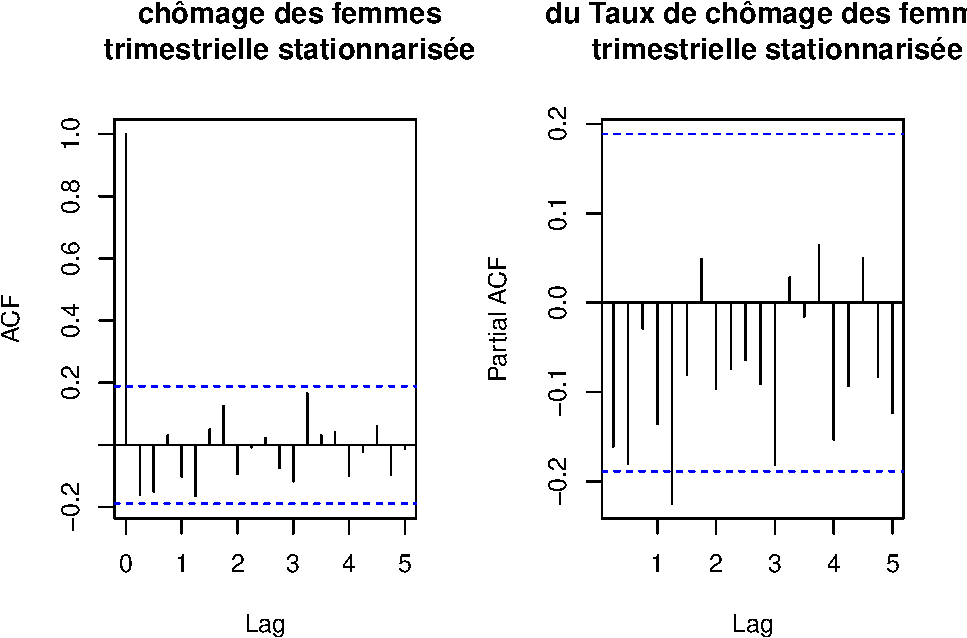
\includegraphics{doc_files/figure-latex/unnamed-chunk-9-1.pdf}
\caption{\label{fig9}}
\end{figure}

\begin{Shaded}
\begin{Highlighting}[]
\NormalTok{corr <-}\StringTok{ }\KeywordTok{cor.mtest}\NormalTok{(trim[}\DecValTok{1}\OperatorTok{:}\DecValTok{109}\NormalTok{,}\OperatorTok{-}\DecValTok{1}\NormalTok{], }\FloatTok{0.95}\NormalTok{)[[}\DecValTok{1}\NormalTok{]]}
\KeywordTok{rownames}\NormalTok{(corr) <-}\StringTok{ }\KeywordTok{c}\NormalTok{(}\StringTok{"MSE"}\NormalTok{,}\StringTok{"PIB"}\NormalTok{,}\StringTok{"SMIC"}\NormalTok{,}\StringTok{"TCHOF"}\NormalTok{)}
\KeywordTok{colnames}\NormalTok{(corr) <-}\StringTok{ }\KeywordTok{c}\NormalTok{(}\StringTok{"MSE"}\NormalTok{,}\StringTok{"PIB"}\NormalTok{,}\StringTok{"SMIC"}\NormalTok{,}\StringTok{"TCHOF"}\NormalTok{)}
\NormalTok{corr}
\end{Highlighting}
\end{Shaded}

\begin{verbatim}
##                MSE          PIB         SMIC        TCHOF
## MSE   0.000000e+00 3.851955e-69 1.436967e-74 3.321841e-12
## PIB   3.851955e-69 0.000000e+00 1.898200e-71 2.387179e-15
## SMIC  1.436967e-74 1.898200e-71 0.000000e+00 1.377731e-10
## TCHOF 3.321841e-12 2.387179e-15 1.377731e-10 0.000000e+00
\end{verbatim}

Nous affichons la matrice des corrélations des différentes variables en
Figure \ref{fig9}. On se rend compte que le taux de chômage des femmes
est corrélé négativement avec toutes les autres variables. Le trio de
variables PIB, masse salariale et SMIC sont extrêmement liées entre
elles. En regardant le tableau des p-values associées au test de Student
(H0 : La corrélation entre les deux variables est nulle), on s'aperçoit
que toutes les variables prises deux à deux présentes une corrélation.

\section{\texorpdfstring{Modélisation individuelle
\label{MI}}{Modélisation individuelle }}\label{modelisation-individuelle}

Une fois que nous avons analysé le comportement des différentes séries
temporelles à notre disposition, nous souhaitons les modéliser afin de
prédire les valeurs futures de ces différentes séries. En effet, si nous
voulons prédire la MSE pour des valeurs futures, nous aurons également
besoin des valeurs associées pour les variables explicatives, qui ne
seront peut-être pas à notre disposition. Nous avons utilisé à la fois
des modèles basés sur un lissage exponentiel et des processus ARMA.

\subsection{Découpage des séries}\label{decoupage-des-series}

Pour chacune des séries, nous allons créer un échantillon
d'apprentissage, qui nous permettra de construire les différents
modèles, ainsi qu'un échantillon de test, qui nous permettra de comparer
les prédictions des modèles construits avec des vraies valeurs.
L'échantillon d'apprentissage sera composé de toutes les valeurs du
premier trimestre 1990 jusqu'au 4e trimestre 2015, tandis que celui de
test comprendra toutes les valeurs à partir du 1er trimestre 2016.

\begin{Shaded}
\begin{Highlighting}[]
\NormalTok{MSETrain <-}\StringTok{ }\KeywordTok{window}\NormalTok{(MSE, }\DataTypeTok{start=}\DecValTok{1990}\NormalTok{, }\DataTypeTok{end=}\KeywordTok{c}\NormalTok{(}\DecValTok{2015}\NormalTok{,}\DecValTok{4}\NormalTok{))}
\NormalTok{MSETest <-}\StringTok{ }\KeywordTok{window}\NormalTok{(MSE, }\DataTypeTok{start=}\DecValTok{2016}\NormalTok{, }\DataTypeTok{end=}\KeywordTok{c}\NormalTok{(}\DecValTok{2017}\NormalTok{,}\DecValTok{2}\NormalTok{))}
\NormalTok{PIBTrain <-}\StringTok{ }\KeywordTok{window}\NormalTok{(PIB, }\DataTypeTok{start=}\DecValTok{1990}\NormalTok{, }\DataTypeTok{end=}\KeywordTok{c}\NormalTok{(}\DecValTok{2015}\NormalTok{,}\DecValTok{4}\NormalTok{))}
\NormalTok{PIBTest <-}\StringTok{ }\KeywordTok{window}\NormalTok{(PIB, }\DataTypeTok{start=}\DecValTok{2016}\NormalTok{, }\DataTypeTok{end=}\KeywordTok{c}\NormalTok{(}\DecValTok{2017}\NormalTok{,}\DecValTok{1}\NormalTok{))}
\NormalTok{SMICTrain <-}\StringTok{ }\KeywordTok{window}\NormalTok{(SMIC, }\DataTypeTok{start=}\DecValTok{1990}\NormalTok{, }\DataTypeTok{end=}\KeywordTok{c}\NormalTok{(}\DecValTok{2015}\NormalTok{,}\DecValTok{4}\NormalTok{))}
\NormalTok{SMICTest <-}\StringTok{ }\KeywordTok{window}\NormalTok{(SMIC, }\DataTypeTok{start=}\DecValTok{2016}\NormalTok{, }\DataTypeTok{end=}\KeywordTok{c}\NormalTok{(}\DecValTok{2017}\NormalTok{,}\DecValTok{2}\NormalTok{))}
\NormalTok{TCHOFTrain <-}\StringTok{ }\KeywordTok{window}\NormalTok{(TCHOF, }\DataTypeTok{start=}\DecValTok{1990}\NormalTok{, }\DataTypeTok{end=}\KeywordTok{c}\NormalTok{(}\DecValTok{2015}\NormalTok{,}\DecValTok{4}\NormalTok{))}
\NormalTok{TCHOFTest <-}\StringTok{ }\KeywordTok{window}\NormalTok{(TCHOF, }\DataTypeTok{start=}\DecValTok{2016}\NormalTok{, }\DataTypeTok{end=}\KeywordTok{c}\NormalTok{(}\DecValTok{2017}\NormalTok{,}\DecValTok{2}\NormalTok{))}
\end{Highlighting}
\end{Shaded}

\subsection{Comparaison des différents
modèles}\label{comparaison-des-differents-modeles}

Afin de comparer les modèles construits pour chaque série avec les
différentes méthodes, nous calculons l'erreur quadratique moyenne (EQM),
soit les moyennes des différences au carré entre les valeurs de test et
les valeurs prédites par le modèle.

\subsection{Lissage exponentiel}\label{lissage-exponentiel}

\subsubsection{Définition}\label{definition}

Le lissage exponentiel permet de prédire les valeurs d'une série
temporelle en lissant successivement les données à partir d'une valeur
initiale. Plus les observations sont éloignées dans le passé, moins leur
poids est important lors du calcul. Pour une série stationnaire, la
formule de calcul d'une valeur est la suivante :
\(s_t = \alpha y_t + (1-\alpha) s_{t-1}\), le paramètre \(\alpha\) étant
le facteur de lissage. Le nom de cette méthode est un lissage
exponentiel \textbf{simple}. Afin de modéliser les séries possédant une
tendance, nous introduisons un paramètre \(\beta\) permettant de la
prendre en compte, la méthode étant appelée lissage exponentiel
\textbf{double}. Enfin, Holt et Winters ont également modifié la méthode
pour qu'elle puisse modéliser les séries comportant une saisonnalité en
introduisant un paramètre \(\gamma\). Ils ont donné leur nom à cette
méthode, qui est donc un lissage exponentiel de \textbf{Holt-Winters}.

Dans notre cas, nous ne calculons pas nous-mêmes \(\alpha\) \(\beta\) et
\(\gamma\) Ces paramètres sont déterminés automatiquement par la
fonction \emph{ets} du package \textbf{forecast} de façon à optimiser la
qualité de la prédiction. Cette fonction permet également de choisir la
méthode à utiliser, grâce à l'argument model. Afin de mesurer la qualité
de notre modèle, nous avons choisi d'utiliser l'\textbf{AICc}(Akaike
Information Criterion with correction). Le choix de l'AICc par rapport à
l'AIC s'explique par le faible nombre de données que nous possédons par
rapport au nombre de paramètres à estimer. C'est ce critère qui nous
servira par la suite afin de comparer nos différents modèles.
\label{AICc}

Prenons l'exemple de la MSE. Nous avons vu dans la partie \ref{MSE} que
la série possédait une tendance linéaire ainsi qu'une saisonnalité
multiplicative. L'argument model de la fonction *ets** prendra donc la
valeur ``ZAM'', (erreur sélectionnée automatiquement, tendance linéaire,
saisonnalité multiplicative). On peut également remarquer que lorsque
tous les paramètres sont automatiquement sélectionnés (valeur ``ZZZ''),
les paramètres retenus sont les mêmes que ceux que nous avions rentré.

\begin{Shaded}
\begin{Highlighting}[]
\NormalTok{LEMSE<-}\KeywordTok{ets}\NormalTok{(MSETrain, }\StringTok{"ZAM"}\NormalTok{)}
\KeywordTok{print}\NormalTok{(LEMSE)}
\end{Highlighting}
\end{Shaded}

\begin{verbatim}
## ETS(M,A,M) 
## 
## Call:
##  ets(y = MSETrain, model = "ZAM") 
## 
##   Smoothing parameters:
##     alpha = 0.7675 
##     beta  = 0.1111 
##     gamma = 0.2325 
## 
##   Initial states:
##     l = 279219343.2211 
##     b = 12053621.0848 
##     s = 1.0092 0.9655 1.0159 1.0094
## 
##   sigma:  0.0279
## 
##      AIC     AICc      BIC 
## 4031.536 4033.451 4055.336
\end{verbatim}

\begin{Shaded}
\begin{Highlighting}[]
\NormalTok{PredLEMSE <-}\StringTok{ }\KeywordTok{forecast}\NormalTok{(LEMSE, }\DataTypeTok{h =} \DecValTok{6}\NormalTok{)}
\KeywordTok{plot}\NormalTok{(MSETest, }\DataTypeTok{main=}\StringTok{"Comparaison entre la prédiction du lissage }
\StringTok{exponentiel et les valeurs réelles pour la masse salariale }
\StringTok{trimestrielle"}\NormalTok{)}
\KeywordTok{lines}\NormalTok{(PredLEMSE}\OperatorTok{$}\NormalTok{mean, }\DataTypeTok{col=}\StringTok{"red"}\NormalTok{)}
\end{Highlighting}
\end{Shaded}

\begin{figure}

{\centering \includegraphics{doc_files/figure-latex/unnamed-chunk-11-1} 

}

\caption{\label{fig10}}\label{fig:unnamed-chunk-11}
\end{figure}

\begin{Shaded}
\begin{Highlighting}[]
\KeywordTok{EQM}\NormalTok{(MSETest, PredLEMSE}\OperatorTok{$}\NormalTok{mean)}
\end{Highlighting}
\end{Shaded}

\begin{verbatim}
## [1] 2.592281e+14
\end{verbatim}

\begin{Shaded}
\begin{Highlighting}[]
\KeywordTok{ets}\NormalTok{(MSETrain, }\StringTok{"ZZZ"}\NormalTok{)}
\end{Highlighting}
\end{Shaded}

\begin{verbatim}
## ETS(M,A,M) 
## 
## Call:
##  ets(y = MSETrain, model = "ZZZ") 
## 
##   Smoothing parameters:
##     alpha = 0.7675 
##     beta  = 0.1111 
##     gamma = 0.2325 
## 
##   Initial states:
##     l = 279219343.2211 
##     b = 12053621.0848 
##     s = 1.0092 0.9655 1.0159 1.0094
## 
##   sigma:  0.0279
## 
##      AIC     AICc      BIC 
## 4031.536 4033.451 4055.336
\end{verbatim}

On obtient donc un AICc de 4033.451 pour le modèle ainsi qu'une erreur
quadratique moyenne de \(2.6*10^{14}\). Le graphique obtenu en figure
\ref{fig10} nous montrent que le modèle obtenu nous donne des
prédictions très proches de la réalité.

\subsubsection{Résultats obtenus}\label{resultats-obtenus}

\begin{Shaded}
\begin{Highlighting}[]
\KeywordTok{par}\NormalTok{(}\DataTypeTok{mfrow=}\KeywordTok{c}\NormalTok{(}\DecValTok{2}\NormalTok{,}\DecValTok{2}\NormalTok{))}
\KeywordTok{plot}\NormalTok{(PIBTest, }\DataTypeTok{ylim=}\KeywordTok{c}\NormalTok{(}\KeywordTok{min}\NormalTok{(PIBTest,PredLEPIB}\OperatorTok{$}\NormalTok{mean),}\KeywordTok{max}\NormalTok{(PIBTest,PredLEPIB}\OperatorTok{$}\NormalTok{mean)), }\DataTypeTok{main=}
\StringTok{"Comparaison entre la prédiction du lissage }
\StringTok{exponentiel et les valeurs réelles pour le PIB }
\StringTok{trimestriel"}\NormalTok{, }\DataTypeTok{cex.main=}\FloatTok{0.8}\NormalTok{)}
\KeywordTok{lines}\NormalTok{(PredLEPIB}\OperatorTok{$}\NormalTok{mean, }\DataTypeTok{col=}\StringTok{"red"}\NormalTok{)}

\KeywordTok{plot}\NormalTok{(SMICTest, }\DataTypeTok{ylim=}\KeywordTok{c}\NormalTok{(}\KeywordTok{min}\NormalTok{(SMICTest,PredLESMIC}\OperatorTok{$}\NormalTok{mean),}\KeywordTok{max}\NormalTok{(SMICTest,PredLESMIC}\OperatorTok{$}\NormalTok{mean)), }
\DataTypeTok{main=}\StringTok{"Comparaison entre la prédiction du lissage }
\StringTok{exponentiel et les valeurs réelles pour le SMIC }
\StringTok{trimestriel"}\NormalTok{, }\DataTypeTok{cex.main=}\FloatTok{0.8}\NormalTok{)}
\KeywordTok{lines}\NormalTok{(PredLESMIC}\OperatorTok{$}\NormalTok{mean, }\DataTypeTok{col=}\StringTok{"red"}\NormalTok{)}

\KeywordTok{plot}\NormalTok{(TCHOFTest, }\DataTypeTok{ylim=}\KeywordTok{c}\NormalTok{(}\KeywordTok{min}\NormalTok{(TCHOFTest,PredLETCHOF}\OperatorTok{$}\NormalTok{mean),}\KeywordTok{max}\NormalTok{(TCHOFTest,PredLETCHOF}\OperatorTok{$}\NormalTok{mean)), }
\DataTypeTok{main=}\StringTok{"Comparaison entre la prédiction du lissage }
\StringTok{exponentiel et les valeurs réelles pour le taux }
\StringTok{de chômage trimestriel"}\NormalTok{, }\DataTypeTok{cex.main=}\FloatTok{0.8}\NormalTok{)}
\KeywordTok{lines}\NormalTok{(PredLETCHOF}\OperatorTok{$}\NormalTok{mean, }\DataTypeTok{col=}\StringTok{"red"}\NormalTok{)}
\end{Highlighting}
\end{Shaded}

\begin{figure}

{\centering 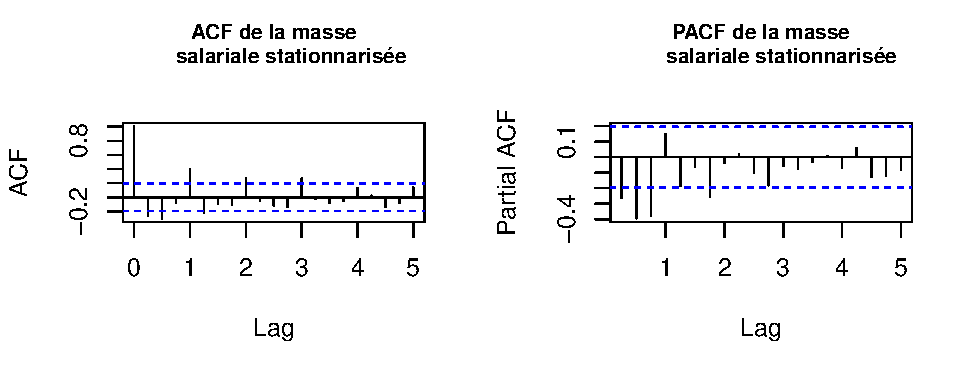
\includegraphics{doc_files/figure-latex/unnamed-chunk-13-1} 

}

\caption{\label{fig11}}\label{fig:unnamed-chunk-13}
\end{figure}

Les graphiques de la figure \ref{fig11} nous montrent des résultats
mitigés. Pour le PIB et le SMIC, les prédictions suivent la forme de la
série mais en sont éloignées. Pour le taux de chômage des femmes, la
méthode de lissage utilisée est un lissage exponentiel simple, ce qui
nous donne donc des prédictions constantes soit de mauvaise qualité.

Nous résumons dans le tableau suivant les résultats obtenus pour chaque
série estimée par un lissage exponentiel.

\begin{longtable}[]{@{}lllll@{}}
\toprule
Variable & Tendance & Saisonnalité & Argument model & AIC\tabularnewline
\midrule
\endhead
MSE & linéaire & multiplicative & ZAM & 4033.45\tabularnewline
PIB & linéaire & absente & ZAN & 2053.15\tabularnewline
SMIC & linéaire & additive & ZAA & -84.96\tabularnewline
TCHOF & absente & absente & ZNN & 204.37\tabularnewline
\bottomrule
\end{longtable}

\subsection{Modèles ARMA}\label{modeles-arma}

\subsubsection{Définition}\label{definition-1}

Les modèles \textbf{ARMA(p,q)} sont une autre famille de modèles
permettant d'estimer une série temporelle. Il est divisé en deux parties
: une partie autorégressive \textbf{AR} auquel est associé un ordre
\emph{p} qui donne le nombre de valeurs passées qui vont être utiles
dans la prédiction, et une partie moyennes mobiles \textbf{MA} qui
permet de de prendre en compte les \emph{q} innovations de la série dans
le futur.

L'une des propriétés des processus ARMA est qu'ils sont utilisés pour
modéliser des séries stationnaires, donc par extension des séries qui ne
possèdent ni tendance ni saisonnalité. Afin de modéliser des séries non
stationnaires, on généralise les processus ARMA en processus
\textbf{ARIMA(p,d,q)}, \emph{d} représentant l'ordre de différenciation
de la série. Les séries saisonnières sont elles modélisées par des
processus \textbf{\(SARIMA(p ,d, q)(P, D, Q)_s\)} qui modélisent des
séries avec une saisonnalité de période \emph{s}.

Comme pour le lissage exponentiel, nous ne calculons pas nous-mêmes les
ordres des processus. Pour cela, la fonction \emph{auto.arima} du
package \textbf{forecast} nous a été très utile. Elle permet en effet de
trouver les ordres du processus qui optimisent un critère défini à
l'avance et de calculer un modèle avec ces coefficients. Nous avons
choisi d'optimiser l'\textbf{AICc}(Akaike Information Criterion with
correction), pour els raisons évoquées dans la partie \ref{AICc}

\begin{Shaded}
\begin{Highlighting}[]
\NormalTok{ARIMAMSE<-}\KeywordTok{auto.arima}\NormalTok{(MSETrain, }\DataTypeTok{ic=}\StringTok{"aicc"}\NormalTok{)}
\KeywordTok{print}\NormalTok{(ARIMAMSE)}
\end{Highlighting}
\end{Shaded}

\begin{verbatim}
## Series: MSETrain 
## ARIMA(0,1,1)(0,1,1)[4] 
## 
## Coefficients:
##           ma1     sma1
##       -0.1986  -0.3857
## s.e.   0.1014   0.0929
## 
## sigma^2 estimated as 7.396e+14:  log likelihood=-1834.54
## AIC=3675.09   AICc=3675.34   BIC=3682.87
\end{verbatim}

\begin{Shaded}
\begin{Highlighting}[]
\NormalTok{PredARIMAMSE<-}\StringTok{ }\KeywordTok{forecast}\NormalTok{(ARIMAMSE, }\DataTypeTok{h=}\DecValTok{6}\NormalTok{)}
\KeywordTok{plot}\NormalTok{(MSETest, }\DataTypeTok{main=}\StringTok{"Comparaison entre le modèle SARIMA et les données de}
\StringTok{    validation pour la masse salariale trimestrielle"}\NormalTok{)}
\KeywordTok{lines}\NormalTok{(PredARIMAMSE}\OperatorTok{$}\NormalTok{mean, }\DataTypeTok{col=}\StringTok{"red"}\NormalTok{)}
\end{Highlighting}
\end{Shaded}

\begin{figure}

{\centering 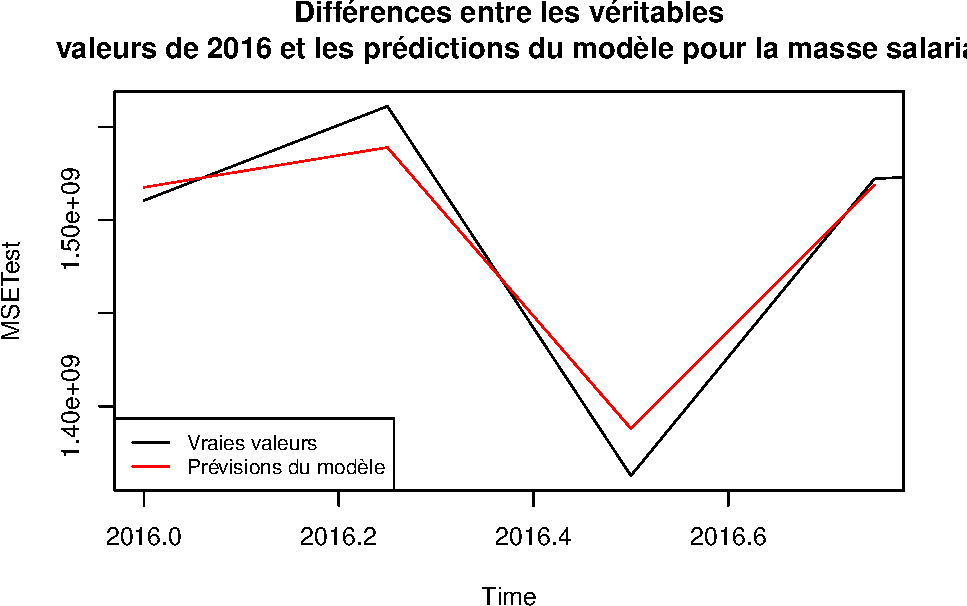
\includegraphics{doc_files/figure-latex/unnamed-chunk-14-1} 

}

\caption{\label{fig12}}\label{fig:unnamed-chunk-14}
\end{figure}

Pour la MSE, on obtient par exemple un modèle \(SARIMA(0,1,1)(0,1,1)_4\)
ainsi qu'un AICc de 3896.01. La figure \ref{fig12} nous donne des
prédictions d'assez bonne qualité mais qui semblent moins bonnes que
celles obtenues par lissage exponentiel.

\subsubsection{Résultats obtenus}\label{resultats-obtenus-1}

\begin{Shaded}
\begin{Highlighting}[]
\KeywordTok{par}\NormalTok{(}\DataTypeTok{mfrow=}\KeywordTok{c}\NormalTok{(}\DecValTok{2}\NormalTok{,}\DecValTok{2}\NormalTok{))}
\NormalTok{ARIMAPIB<-}\KeywordTok{auto.arima}\NormalTok{(PIBTrain, }\DataTypeTok{ic=}\StringTok{"aicc"}\NormalTok{, }\DataTypeTok{seasonal=}\NormalTok{F)}
\KeywordTok{print}\NormalTok{(ARIMAPIB)}
\end{Highlighting}
\end{Shaded}

\begin{verbatim}
## Series: PIBTrain 
## ARIMA(2,1,0) with drift 
## 
## Coefficients:
##          ar1     ar2      drift
##       0.4701  0.1596  1585.8365
## s.e.  0.0966  0.0966   456.3009
## 
## sigma^2 estimated as 3153980:  log likelihood=-915.48
## AIC=1838.95   AICc=1839.36   BIC=1849.49
\end{verbatim}

\begin{Shaded}
\begin{Highlighting}[]
\NormalTok{PredARIMAPIB<-}\StringTok{ }\KeywordTok{forecast}\NormalTok{(ARIMAPIB, }\DataTypeTok{h=}\DecValTok{5}\NormalTok{)}
\KeywordTok{plot}\NormalTok{(PIBTest, }\DataTypeTok{ylim=}\KeywordTok{c}\NormalTok{(}\KeywordTok{min}\NormalTok{(PIBTest,PredARIMAPIB}\OperatorTok{$}\NormalTok{mean),}\KeywordTok{max}\NormalTok{(PIBTest,PredARIMAPIB}\OperatorTok{$}\NormalTok{mean)), }
\DataTypeTok{main=}\StringTok{"Comparaison entre le modèle SARIMA et les données de}
\StringTok{    validation pour le PIB trimestriel"}\NormalTok{, }\DataTypeTok{cex.main=}\FloatTok{0.8}\NormalTok{)}
\KeywordTok{lines}\NormalTok{(PredARIMAPIB}\OperatorTok{$}\NormalTok{mean, }\DataTypeTok{col=}\StringTok{"red"}\NormalTok{)}

\NormalTok{ARIMASMIC<-}\KeywordTok{auto.arima}\NormalTok{(SMICTrain, }\DataTypeTok{ic=}\StringTok{"aicc"}\NormalTok{)}
\KeywordTok{print}\NormalTok{(ARIMASMIC)}
\end{Highlighting}
\end{Shaded}

\begin{verbatim}
## Series: SMICTrain 
## ARIMA(1,0,0)(1,1,0)[4] with drift 
## 
## Coefficients:
##          ar1     sar1   drift
##       0.8645  -0.3643  0.0486
## s.e.  0.0514   0.0961  0.0080
## 
## sigma^2 estimated as 0.003998:  log likelihood=134.95
## AIC=-261.89   AICc=-261.47   BIC=-251.47
\end{verbatim}

\begin{Shaded}
\begin{Highlighting}[]
\NormalTok{PredARIMASMIC<-}\StringTok{ }\KeywordTok{forecast}\NormalTok{(ARIMASMIC, }\DataTypeTok{h=}\DecValTok{6}\NormalTok{)}
\KeywordTok{plot}\NormalTok{(SMICTest, }\DataTypeTok{ylim=}\KeywordTok{c}\NormalTok{(}\KeywordTok{min}\NormalTok{(SMICTest,PredARIMASMIC}\OperatorTok{$}\NormalTok{mean),}\KeywordTok{max}\NormalTok{(SMICTest,PredARIMASMIC}\OperatorTok{$}\NormalTok{mean)), }
\DataTypeTok{main=}\StringTok{"Comparaison entre le modèle SARIMA et les données de}
\StringTok{    validation pour le SMIC trimestriel"}\NormalTok{, }\DataTypeTok{cex.main=}\FloatTok{0.8}\NormalTok{)}
\KeywordTok{lines}\NormalTok{(PredARIMASMIC}\OperatorTok{$}\NormalTok{mean, }\DataTypeTok{col=}\StringTok{"red"}\NormalTok{)}

\NormalTok{ARIMATCHOF<-}\KeywordTok{auto.arima}\NormalTok{(TCHOFTrain, }\DataTypeTok{ic=}\StringTok{"aicc"}\NormalTok{, }\DataTypeTok{seasonal=}\NormalTok{F)}
\KeywordTok{print}\NormalTok{(ARIMATCHOF)}
\end{Highlighting}
\end{Shaded}

\begin{verbatim}
## Series: TCHOFTrain 
## ARIMA(1,1,1) 
## 
## Coefficients:
##          ar1      ma1
##       0.6974  -0.5005
## s.e.  0.1669   0.1935
## 
## sigma^2 estimated as 0.06173:  log likelihood=-1.76
## AIC=9.52   AICc=9.76   BIC=17.42
\end{verbatim}

\begin{Shaded}
\begin{Highlighting}[]
\NormalTok{PredARIMATCHOF<-}\StringTok{ }\KeywordTok{forecast}\NormalTok{(ARIMATCHOF, }\DataTypeTok{h=}\DecValTok{6}\NormalTok{)}
\KeywordTok{plot}\NormalTok{(TCHOFTest, }\DataTypeTok{main=}\StringTok{"Comparaison entre le modèle SARIMA et les données de}
\StringTok{    validation pour le taux de chômage des femmes trimestriel"}\NormalTok{, }\DataTypeTok{cex.main=}\FloatTok{0.8}\NormalTok{)}
\KeywordTok{lines}\NormalTok{(PredARIMATCHOF}\OperatorTok{$}\NormalTok{mean, }\DataTypeTok{col=}\StringTok{"red"}\NormalTok{)}
\end{Highlighting}
\end{Shaded}

\begin{figure}
\centering
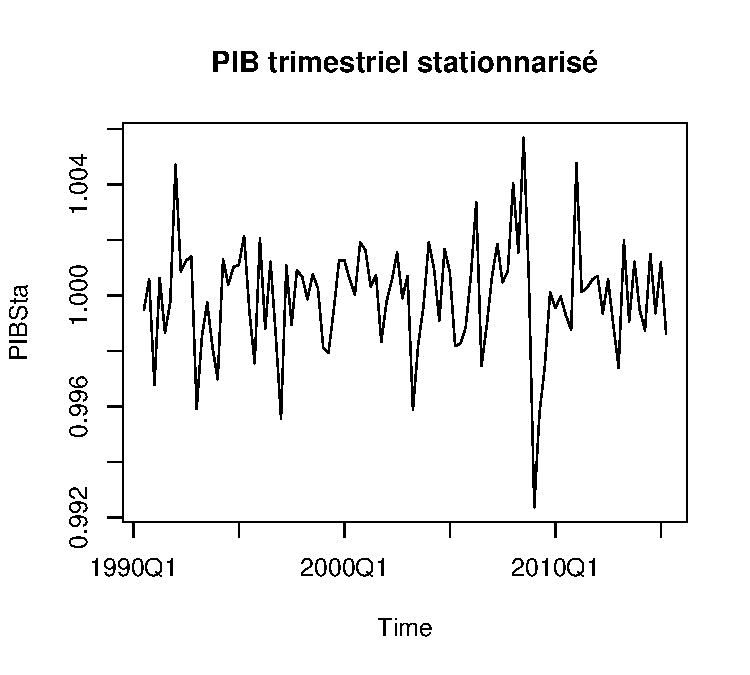
\includegraphics{doc_files/figure-latex/unnamed-chunk-15-1.pdf}
\caption{\label{fig13}}
\end{figure}

Comme pour le lissage exponentiel, nous résumons les résultats obtenus
dans un tableau pour plus de lisibilité. Le PIB et le taux de chômage
des femmes ne comportent pas de partie saisonnière car comme vu dans les
parties \ref{PIB} et \ref{TCHOF} on ne constate pas de saisonnalité dans
l'analyse descriptive de la série. On peut également voir sur la figure
\ref{fig13} que les prédictions du PIB semblent de bien meilleure
qualité

\begin{longtable}[]{@{}lll@{}}
\toprule
Variable & Ordre du processus & AICc\tabularnewline
\midrule
\endhead
MSE & (0,1,1)(0,1,1) & 3675.34\tabularnewline
PIB & (2,1,0) & 1839.36\tabularnewline
SMIC & (1,0,0)(1,1,0) & -261.47\tabularnewline
TCHOF & (0,1,1) & 9.76\tabularnewline
\bottomrule
\end{longtable}

\subsection{Comparaison des différents
modèles}\label{comparaison-des-differents-modeles-1}

Une fois que nous avons construit les deux types de modèles pour chacune
des variables, nous souhaitons les comparer pour savoir quel modèle est
le plus efficace pour prédire chacune des variables. Pour cela, les EQM,
calculant l'erreur de prédiction, de chacun des modèles sont
synthétisées dans le tableau suivant. L'AICc ne peut pas être utilsié
ici car les méthodes à comparer sont différentes. Il n'est donc pas sûr
que la méthode utilisée pour calculer la vraisemblance soit la même.

\begin{Shaded}
\begin{Highlighting}[]
\NormalTok{resultats<-}\KeywordTok{matrix}\NormalTok{(}\DataTypeTok{nrow=}\DecValTok{4}\NormalTok{, }\DataTypeTok{ncol=}\DecValTok{2}\NormalTok{, }\DataTypeTok{dimnames =} \KeywordTok{list}\NormalTok{(}\KeywordTok{c}\NormalTok{(}\StringTok{"MSE"}\NormalTok{, }\StringTok{"PIB"}\NormalTok{, }\StringTok{"SMIC"}\NormalTok{, }\StringTok{"TCHOF"}\NormalTok{), }
                                                  \KeywordTok{c}\NormalTok{(}\StringTok{"lissage"}\NormalTok{, }\StringTok{"ARMA"}\NormalTok{)))}
\NormalTok{resultats[}\DecValTok{1}\NormalTok{,}\DecValTok{1}\NormalTok{] =}\StringTok{ }\KeywordTok{EQM}\NormalTok{(MSETest, PredLEMSE}\OperatorTok{$}\NormalTok{mean)}
\NormalTok{resultats[}\DecValTok{2}\NormalTok{,}\DecValTok{1}\NormalTok{] =}\StringTok{ }\KeywordTok{EQM}\NormalTok{(PIBTest, PredLEPIB}\OperatorTok{$}\NormalTok{mean)}
\NormalTok{resultats[}\DecValTok{3}\NormalTok{,}\DecValTok{1}\NormalTok{] =}\StringTok{ }\KeywordTok{EQM}\NormalTok{(SMICTest, PredLESMIC}\OperatorTok{$}\NormalTok{mean)}
\NormalTok{resultats[}\DecValTok{4}\NormalTok{,}\DecValTok{1}\NormalTok{] =}\StringTok{ }\KeywordTok{EQM}\NormalTok{(TCHOFTest, PredLETCHOF}\OperatorTok{$}\NormalTok{mean)}
\NormalTok{resultats[}\DecValTok{1}\NormalTok{,}\DecValTok{2}\NormalTok{] =}\StringTok{ }\KeywordTok{EQM}\NormalTok{(MSETest, PredARIMAMSE}\OperatorTok{$}\NormalTok{mean)}
\NormalTok{resultats[}\DecValTok{2}\NormalTok{,}\DecValTok{2}\NormalTok{] =}\StringTok{ }\KeywordTok{EQM}\NormalTok{(PIBTest, PredARIMAPIB}\OperatorTok{$}\NormalTok{mean)}
\NormalTok{resultats[}\DecValTok{3}\NormalTok{,}\DecValTok{2}\NormalTok{] =}\StringTok{ }\KeywordTok{EQM}\NormalTok{(SMICTest, PredARIMASMIC}\OperatorTok{$}\NormalTok{mean)}
\NormalTok{resultats[}\DecValTok{4}\NormalTok{,}\DecValTok{2}\NormalTok{] =}\StringTok{ }\KeywordTok{EQM}\NormalTok{(TCHOFTest, PredARIMATCHOF}\OperatorTok{$}\NormalTok{mean)}
\NormalTok{resultats}
\end{Highlighting}
\end{Shaded}

\begin{verbatim}
##            lissage         ARMA
## MSE   2.592281e+14 3.060118e+14
## PIB   5.885443e+06 8.892292e+05
## SMIC  3.371267e-03 8.609164e-03
## TCHOF 5.833300e-02 6.223076e-02
\end{verbatim}

Nous nous rendons compte que le lissage a une EQM plus faible pour la
masse salariale (notre variable d'intérêt), ainsi que pour le SMIC et le
taux de chômage des femmes. En ce qui concerne le PIB, le modèle ARIMA
est plus performant. Cette analyse va nous servir par la suite, comme
expliqué au début de la partie \ref{MI}

\subsection{Estimation de la valeur manquante du
PIB}\label{estimation-de-la-valeur-manquante-du-pib}

Contrairement aux autres variables, nous n'avons à notre disposition
pour le PIB que les valeurs jusqu'au premier trimestre de 2017. Ceci
nous impose de négliger la dernière valeur de toutes les autres séries
pour que toutes les variables soient étudiées sur la même période. Pour
éviter ce problème, nous décidons d'estimer la variable du PIB pour le
2e trimestre de 2017. Afin de faire cela, nous allons utiliser la valeur
estimée par le modèle SARIMA correspondant à la variable PIB, étant
donné que c'est celui qui donnait les meilleures prédictions.

\begin{Shaded}
\begin{Highlighting}[]
\NormalTok{PredARIMAPIB<-}\StringTok{ }\KeywordTok{forecast}\NormalTok{(ARIMAPIB, }\DataTypeTok{h=}\DecValTok{6}\NormalTok{)}
\NormalTok{new.value <-}\StringTok{ }\NormalTok{PredARIMAPIB}\OperatorTok{$}\NormalTok{mean[}\DecValTok{6}\NormalTok{]}
\NormalTok{PIBTest<-}\KeywordTok{ts}\NormalTok{(}\KeywordTok{c}\NormalTok{(PredARIMAPIB}\OperatorTok{$}\NormalTok{mean, new.value), }\DataTypeTok{start =} \DecValTok{2016}\NormalTok{, }\DataTypeTok{end =} \KeywordTok{c}\NormalTok{(}\DecValTok{2017}\NormalTok{, }\DecValTok{2}\NormalTok{), }\DataTypeTok{frequency=}\DecValTok{4}\NormalTok{)}
\end{Highlighting}
\end{Shaded}

\section{Modélisation ARMA avec variables
exogènes}\label{modelisation-arma-avec-variables-exogenes}

\subsection{Définition}\label{definition-2}

Maintenant que nous avons modélisé chaque série individuellement, nous
souhaitons savoir s'il est possible d'améliorer la qualité de prédiction
des séries MSE annuelle et trimestrielle à l'aide des autres variables à
notre disposition. Pour ce faire, nous allons construire des lissages et
des modèles SARIMA prenant en compte des variables exogènes.

\$ (y\_t - \mu - X\_t'\beta) = \phi\emph{1(y}\{t-1\} - \mu -
X\_\{t-1\}`\beta) + \ldots{} + \phi\emph{p(y}\{t-p\} - \mu -
X\_\{t-p\}')\$ \$ + \epsilon\_t + \theta\emph{1\epsilon}\{t-1\} +
\ldots{} + \theta\emph{q\epsilon}\{t-q\} \$

\(X_t'\) est un vecteur contenant les valeurs des variables exogènes à
l'instant \(t\). \(\beta\) est un vecteur contenant les coefficients
liés à ces variables.

\subsection{Résultats obtenus}\label{resultats-obtenus-2}


\end{document}
